\documentclass[12pt]{article}

\usepackage{amsthm}
\usepackage{amsmath}
\usepackage{amsfonts}
\usepackage{graphicx}
\graphicspath{ {images/}{figs/} }
\usepackage{listings}
\lstset{
  basicstyle=\ttfamily,
  columns=fullflexible,
  frame=single,
  breaklines=true,
}

\theoremstyle{definition}
\newtheorem{definition}{Definition}

\title{{\small{Machine Learning and Algorithms for Data Mining} \\
Assessment 2\footnote{Word count: 2467 --- Computed using TexCount}} \\
\textit{Analysis of graph-structured data}}
\author{Sebastian Borgeaud --- spb61@cam.ac.uk}

\begin{document}
\maketitle

\begin{abstract}
	In this report I explore the efficiency of various algorithms on the task of transductive classification on a graph. In particular, I focus on the cora dataset, consisting of 2078 scientific publications each classified into one of seven classes. Each publication is described by a bag-of-word vector for a vocabulary of 1433 unique words. The edges in the graph represent citations (REFERENCE).
	\end{abstract}

\section{Main contributions, Key Concepts and Ideas}

TODO: Background / Related work

\subsection{Introduction}
Many real world datasets occur naturally in the form of graphs, for example protein-protein interaction networks in biology, social networks in social sciences and relational databases to name just a few examples from different fields. (CITATIONS) In this report I focus on the problem of node classification in the transductive setting. At training time, the entire structure of the network is known but only few nodes are labelled. At test time, we wish to infer the labels of some or all of the remaining nodes. This differs from supervised learning in two ways: i) the data points (the nodes) are connected to each other and ii) the features of the nodes that will be classified at test time are known in advance, i.e. the graph is known at test time. 
Instead, the problem can be seen as a graph-based semi-supervised learning problem, where the label information is smoothed over the graph via some form of explicit graph-based regularisation. For example, we could make the assumption that adjacent nodes are more likely to have the same class label and incorporate this in the loss
\begin{equation}
	\mathcal{L} = \mathcal{L}_0 + \lambda \mathcal{L}_{\mathit{reg}}
\end{equation}
where $\mathcal{L}_0$ is some supervised loss w.r.t to labeled nodes and $\mathcal{L}_{\mathit{reg}}$ is a graph Laplacian regularisation term using the made assumption.

\subsection{Dataset}
I focus on the cora dataset, consisting of 2078 machine learning publications, each representing a node in the graph (REFERENCE). Each publication is classified into one of seven classes: `Case Based', `Genetic Algorithms', `Neural Networks', `Probabilistic Methods', `Reinforcement Learning', `Rule Learning' or `Theory'. Each publication has a binary bag-of-word feature vector for a vocabulary of 1433 unique words. The edges are directed (WRONG, adj.transpose == adj) and represent citations, where an edge $\mathit{pub_1} \to \mathit{pub_2}$ means that publication $\mathit{pub_2}$ is cited in publication $\mathit{pub_1}$. The papers were selected in such a way that every paper cites or is cited by at least one other paper.

In particular, I use the data split introduced by Kipf and Welling \cite{kipf2017semi}. At training time the label of only 140 nodes is given (about 6.7\%). A further 500 node labels are given as validation data. We wish to infer the label of 1000 nodes not contained in either the test or validation set. Furthermore, the edge orientations are ignored by constructing a symmetric adjacency matrix.

The distribution of node degrees is plotted in figures \ref{fig/node_degrees} and \ref{fig/node_degrees_truncated}. Most nodes have few outgoing edges, with 59.9\% of the nodes having 3 outgoing edges or less and over 96.5\% having 10 or fewer. There seems to be one extreme outlier publication making 168 citations, whereas the second most citing paper makes only 78 citations.

\begin{figure}[h]
	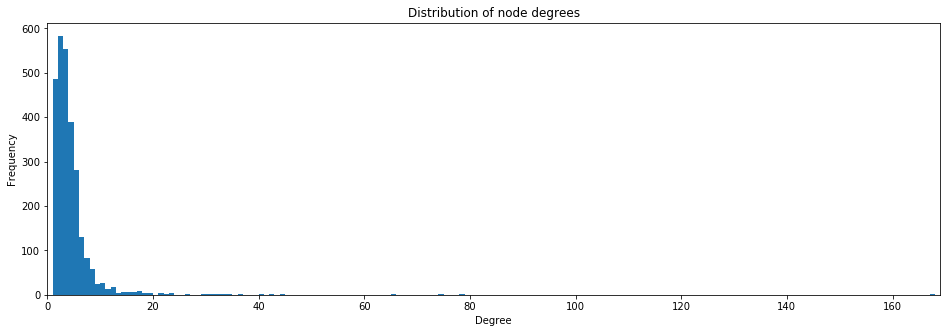
\includegraphics[width=1.0\textwidth]{node_degrees}
	\centering
	\caption{Distribution of node degrees in Cora dataset}
	\label{fig/node_degrees}
\end{figure}

\begin{figure}[h]
	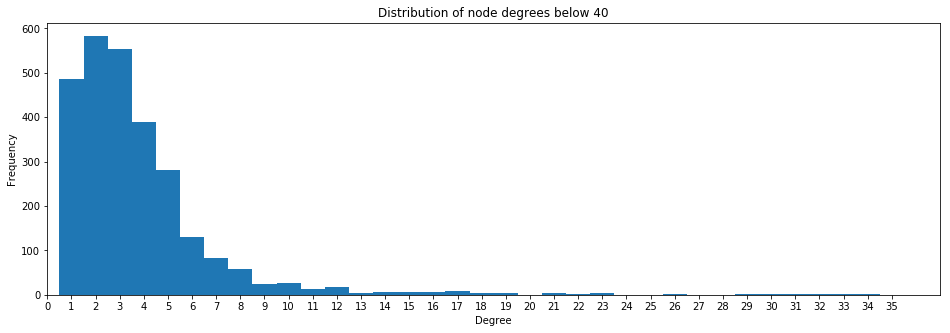
\includegraphics[width=1.0\textwidth]{node_degrees_truncated}
	\centering
	\caption{Distribution of node degrees for nodes with degree below 40. This includes 2701 of the 2708 publications, or above 99.7\% of the nodes.}
	\label{fig/node_degrees_truncated}
\end{figure}

\section{Methods}
\subsection{SVM on features alone}
First, I create a simple baseline model by training an SVM on the features of the nodes only, i.e.\ the bag-of-words vectors of the publications. This approach ignores the structure of the graph entirely and is therefore an instance of a supervised learning problem. In particular, given a bag-of-word representation of a publication we wish to infer its publication type. 

I trained the SVM on the training instances of the dataset. The trained model is then used to predict the class labels of the test publications. The model hyper-parameters are optimised using the validation data set. For the kernel I considered both a linear and a radial basis function.

\subsection{SVM with neighbour features}
Next, I incorporate some information about the graph structure into the SVM model. To do this I combine the features of the neighbours of a node by taking their average and concatenating the resulting feature vector to the feature vector of the node itself. That is, we train the SVM on the features $x'$ where for each node $i$,
\[
	x'^{(i)} = \big[x^{(i)} || x_{neighbours}^{(i)} \big]
\]
where
\[
	x_{neighbours}^{(i)} = \frac{1}{\left\vert \mathcal{N}(i) \right\vert} \sum_{j \in N(i)} x^{(j)}
\]
where $N(i)$ is the set of neighbour nodes of node $i$.

\subsection{Feedforward neural network with neighbour features}
Next, I train a simple feedforward neural network on the simple concatenation of the node features with the average of the features of the neigbouring nodes. The network consists of two fully-connected layers. The first layer consists of 64 hidden units and has a ReLU activation function. The second layer consists of 7 output units, to which is applied a softmax activation to obtain a probability distribution over the 7 classes. Furthermore, as the number of training data is very small, I make use of heavy regularisation using Dropout \cite{srivastava2014dropout} on both the input layer and on the output of the first hidden layer. I also add an L2 regularisation cost on the weights of the first hidden layer.

\subsection{Graph Convolutional Network}
The third algorithm I tested on this dataset is the Graph Convolutional Network, presented by Kipf and Welling \cite{kipf2017semi}. The graph structure is encoded directly using a neural network $f(X, A)$ where $X$ is an NxF matrix containing in each row $i$ the features for node $i$ and $A$ is the NxN adjacency matrix. The model is trained on a supervised loss $\mathcal{L}_0$. This allows the model to distribute the gradient information from $\mathcal{L}_0$ to all nodes and therefore learn representations for nodes with and without labels \cite{kipf2017semi}.

\bigskip

A Graph Convolutional Network (GCN) is a neural network with the following layer-wise propagation rule, where the activations in each layer $H^{(l)}$ are computed as
\[
H^{(l+1)} = \sigma \big( \tilde{D}^{-\frac{1}{2}} \tilde{A} \tilde{D}^{-\frac{1}{2}} H^{(l)} W^{(l)}\big)
\]
Here, $\tilde{A} = A + I_n$ is the adjacency matrix with self-connections, hence adding the identity matrix $I_n$. $\tilde{D}$ is the diagonal degree matrix of $\tilde{A}$, that is $\tilde{D}_{ii} = \sum_{j} \tilde{A}_{ij}$. $W^{(l)}$ are the trainable neural network weights in layer $l$. Finally, $\sigma(\cdot)$ is an activation function.

\bigskip

For the cora dataset, the authors present a 2 layer GCN with a ReLU activation in the first layer and a softmax activation in the second layer. The computation of the forward pass of the neural network can therefore be described concisely as
\[
f(X,A) = \textrm{softmax}\big(\hat{A}\ \textrm{ReLU}\big( \hat{A} X W^{(0)} \big)\ W^{(1)} \big)
\]
where $\hat{A} = \tilde{D}^{-\frac{1}{2}} \tilde{A} \tilde{D}^{-\frac{1}{2}}$ and can be precomputed in a pre-processing step. $W^{(0)}$ is an $\textrm{N} \times \textrm{H}$ weight matrix of reals, where H is the number of nodes in the hidden layer and $W^{(1)}$ is an $\textrm{H} \times \textrm{C}$ weight matrix, where C is the number of classes, i.e.\ 7  for the Cora dataset. The ReLU activation function just clips the input to 0,
\[
\textrm{ReLU}(x) = \max(0, x)
\]
and the softmax activation computes for each component $x_i$
\[
\textrm{softmax}(x_i) = \frac{\exp(x_i)}{\sum_j \exp(x_j)}
\]
During training the cross-entropy loss 
\[
\mathcal{L} = - \sum_{l \in \textrm{y}_L} \sum_{c=1}^{C} Y_{lc} \ln f(X,A)_{lc}
\]
is minimised over all labeled examples $\textbf{y}_L$ using gradient descent. As the entire dataset fits in memory, we can use a single batch containing the entire network. Furthermore, dropout \cite{srivastava2014dropout} is added to the input features and to the output of the first layer.

\subsection{Graph Attention Networks}
Next, I implemented the Graph Attention Networks (GAT) algorithm presented by Veli{\v{c}}kovi{\'{c}} et al.\ \cite{velickovic2018graph}. Attention mechanism have become widely popular and have achieved state-of-the-art results in sequence-based tasks, see for example Bahdanau et al.\ (2014) \cite{bahdanau2014neural} or Vaswani et al.\ (2017) \cite{vaswani2017attention}. Attention mechanism have the advantage of giving the neural network the ability to learn on which part of the input to focus. In the GAT case, we talk about self-attention because the attention mechanism is used to compute a representation of a single sequence. The main idea is to compute a hidden representation for each node in the graph by attending over all its neighbours using self-attention.

\bigskip

The GAT architecture is best described in terms of its layers, called graph attention layers. In each layer, the input features $\textbf{X}$ are linearly transformed into $\textbf{X}' = \textbf{X}\textbf{W}$ where $W$ is a $\textrm{F} \times \textrm{F}'$ weight matrix. Thus each node feature vector $h_i = X_i$ is linearly transformed to a feature vector $h'_i = X'_i = h_i \textbf{W}$ of length $F'$. Then, self-attention is performed on the nodes, based on a shared attentional mechanism, a function $a: \mathbb{R}^{F'} \times \mathbb{R}^{F'} \to \mathbb{R}$ mapping two transformed input feature vectors to a real attention coefficient:
\[
e_{ij} = a(h'_i, h'_j) = a(h_i \textbf{W}, h_j \textbf{W})
\]

Intuitively, $e_{ij}$ indicates how important the features of node $j$ are to node $i$. To inject graph structural information, we only attend over the some neighbourhood $\mathcal{N}(i)$ for a given node $i$, defined to be the direct neighbours of $i$, including $i$ itself. Hence, we have that
\begin{equation*}
e_{ij} = \begin{cases}
				a(h_i \textbf{W}, h_j \textbf{W}) &\text{if $A_{ij} = 1$}\\
				0 &\text{otherwise}
			\end{cases}
\end{equation*}
Then, the coefficients are normalised using the softmax function:
\[
\alpha_{ij} = \textrm{softmax}(e_{ij}) = \frac{\exp(e_{ij})}{\sum_{k \in \mathcal{N}(i)} \exp(e_{ik})}
\]
Here, the attention mechanism is defined to be a single-layer neural network, parametrised by weights $\textbf{a}$ and using a LeakyReLU activation: 
\[
\textrm{LeakyReLU}_{\alpha}(x) = 
	\begin{cases}
		x &\text{if $x \ge 0$}\\
		\alpha x &\text{otherwise}
	\end{cases}
\]
The attention coefficients can therefore be described concisely as
\[
\alpha_{ij} = \frac{\exp \big( \textrm{LeakyReLU}\big( \textbf{a}^T \big[ h_i \textbf{W} \vert\vert h_j \textbf{W} \big] \big) \big)}
{
\sum_{k \in \mathcal{N}(i)} \exp \big( \textrm{LeakyReLU}\big( \textbf{a}^T \big[ h_i \textbf{W} \vert\vert h_k \textbf{W} \big] \big) \big)
}
\]
Next, we use the attention coefficients to compute a linear combination of the transformed features and then applying a nonlinearity. This gives the output of a graph attention layer
\[
g_i = \sigma \big( \sum_{j \in \mathcal{N}(i)} \alpha_{ij} h_j \textbf{W} \big)
\]
Furthermore, we can apply multi-head attention to stabilise the learning process. Instead of using a single attention mechanism, we use $K_a$ simultaneously but independently, concatenating their output:
\[
g_i = {\Big\vert\Big\vert}_{k=1}^{K_a} \sigma \big( \sum_{j \in \mathcal{N}(i)} \alpha_{ij}^k h_j \textbf{W}^k \big)
\]
Note that in this case the ouput feature vectores will have size $K_a F'$.
\section{Results \& analysis}

\section{Conclusion}

\bibliography{bib}
\bibliographystyle{unsrt}


\end{document}